\documentclass[11pt]{article}
\usepackage{booktabs}
\usepackage{natbib}
\usepackage{fullpage}
\usepackage{fancyhdr}

\usepackage{amsmath}
\usepackage{amssymb}
\usepackage{url}

\usepackage{listings}
\usepackage{color}
\lstset{language=Python,
        basicstyle=\footnotesize\ttfamily,
        showspaces=false,
        showstringspaces=false,
        tabsize=2,
        breaklines=false,
        breakatwhitespace=true,
        identifierstyle=\ttfamily,
        keywordstyle=\color[rgb]{0,0,1},
        commentstyle=\color[rgb]{0.133,0.545,0.133},
        stringstyle=\color[rgb]{0.627,0.126,0.941},
    }

\usepackage{graphicx}

% header
\fancyhead{}
\fancyfoot{}
\fancyfoot[C]{\thepage}
\fancyhead[R]{Daniel Foreman-Mackey}
\fancyhead[L]{Statistical Natural Language Processing --- Homework 4}
\pagestyle{fancy}
\setlength{\headsep}{10pt}
\setlength{\headheight}{20pt}

% shortcuts
\newcommand{\Eq}[1]{Equation (\ref{eq:#1})}
\newcommand{\eq}[1]{Equation (\ref{eq:#1})}
\newcommand{\eqlabel}[1]{\label{eq:#1}}
\newcommand{\Fig}[1]{Figure~\ref{fig:#1}}
\newcommand{\fig}[1]{Figure~\ref{fig:#1}}
\newcommand{\figlabel}[1]{\label{fig:#1}}

\newcommand{\etal}{\emph{et al.}}

\newcommand{\pr}[1]{\ensuremath{p\left (#1 \right )}}
\newcommand{\lk}[1]{\ensuremath{\mathcal{L} \left ( #1 \right )}}
\newcommand{\bvec}[1]{\ensuremath{\boldsymbol{#1}}}
\newcommand{\dd}{\ensuremath{\, \mathrm{d}}}
\newcommand{\normal}[2]{\ensuremath{\mathcal{N} \left ( #1; #2 \right ) }}
\newcommand{\T}{^\mathrm{T}}

\newcommand{\data}{\mathcal{D}}
\newcommand{\code}[1]{{\sffamily #1}}
\DeclareMathOperator*{\argmax}{arg\,max}


\begin{document}

I implemented this assignment in pure Python (using extensive use of NumPy for
vectorized operations) and, as you'll see below, I was able to scale the
training to about 250k training sentences.
To go much further than that, further optimizations would be necessary but
this level seemed acceptable for this context.
All of the code that I used for this assignment and the source code for this
document is available on GitHub at \url{https://github.com/dfm/nlp}.

\section{Introduction}

The problem that we're trying to solve in this assignment is word alignment:
given two sentences---one in French and one in English---what is the most
probable set of correspondences between the words.
More concretely, the mathematical quantity of interest is
\begin{eqnarray}\eqlabel{prob}
    p (\bvec{f},\,\bvec{a}\,|\,\bvec{e})\quad,
\end{eqnarray}
the joint probability of a French sentence $\bvec{f}$ (with $m$ words) and
``alignment vector'' $\bvec{a}$ given the English sentence $\bvec{e}$ (with
$l$ words).
In particular, the test that we will implement is based on the maximum
a posteriori alignment $\hat{\bvec{a}}$
\begin{eqnarray}
\hat{\bvec{a}} &=& \argmax_a p (\bvec{f},\,\bvec{a}\,|\,\bvec{e}) \quad.
\end{eqnarray}
This quantity is used in machine translation because in that problem, you
would want to train a model for
\begin{eqnarray}
p(\bvec{e}\,|\,\bvec{f}) &\propto&
    p(\bvec{e})\,p(\bvec{f}\,|\,\bvec{e}) \nonumber\\
    &=& p(\bvec{e})\,
        \sum_a p (\bvec{f},\,\bvec{a}\,|\,\bvec{e}) \quad.
\end{eqnarray}
The \emph{alignment vector} $\bvec{a}$ is a list of integers (of length $m$)
that map positions in $\bvec{f}$ to positions in $\bvec{e}$.
For example, \fig{blue-house} shows two possible alignments between the
sentences $\bvec{e} = blue_1\,house_2$ and
$\bvec{f} = la_1\,maison_2\,bleu_3$.
The left panel shows the alignment associated with the vector
$\bvec{a} = \{-1,\,1,\,2\}$ and the right panel shows $\bvec{a} =
\{-1,\,2,\,1\}$ where $a_i=-1$ indicates the \code{NULL} alignment.

\begin{figure}[htbp]
\begin{center}
    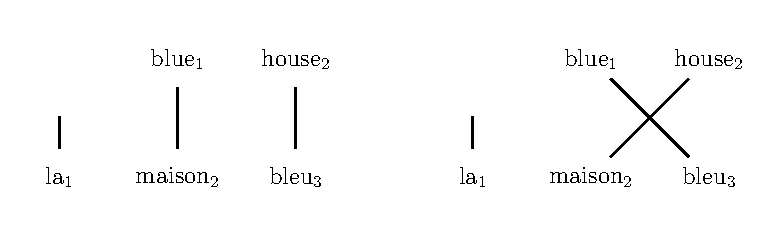
\includegraphics{fig1.pdf}
\end{center}
\caption{%
An example of the possible alignment vectors in a simple sentence pair.
The top line gives the English sentence and the bottom is the French and the
edges indicate the alignment.
\figlabel{blue-house}}
\end{figure}

In this assignment, I'll implement three learning algorithms for \eq{prob}
based on three different sets of independence assumptions.
The first model is based on very simple word-level heuristics and the
following two are the two simplest probabilistic generative models from
\citet{ibm}.

\section{Evaluating Performance}

\section{Baseline Model}

The baseline model is a diagonal alignment $\hat{\bvec{a}} = \{a_i =
i,\,\mathrm{for}\,i=1,\,\cdots,\,m\}$.
For comparison, this model achieves a precision of 33.5\%, a recall of 19.8\%
and an AER of 71.2\% on the provided validation set.
We can also run this model on the provided \code{miniTest} dataset and find a
precision and recall of 88.9\% and an AER of 11.1\%.

\section{Heuristic Model}

The first more sophisticated model that we were to implement is a model based
on some sort of word-level heuristics.
I chose to use word co-occurrence rates as the heuristic.
In practice, this means that
\begin{eqnarray}
p(\bvec{f},\,\bvec{a}\,|\,\bvec{e}) &=&
    \prod_{i=1}^m \frac{c(f_i,\,e_{a_i})}{c(f_i)\,c(e_{a_i})} \quad.
\end{eqnarray}
where $c(f_i,\,e_{a_i})$ is the number of times that both $f_i$ and $e_{a_i}$
appear together in a sentence pair and $c(f_i)$ and $c(e_{a_i})$ are the
total number of times that $f_i$ and $e_{a_i}$, respectively, appear in the
training data.
The only complication in this model comes when an unknown French word appears.
I chose to deal with this by falling back on the baseline (diagonal) alignment
for these unknown words.

On the \code{miniTest}, this model gives a precision of 81.8\%, a perfect
recall and an AER of 10\%.
For the validation data, the results (as a function of the number of training
sentence pairs used) are shown in Table~\ref{tab:heuristic} and
\fig{heuristic}.
Given the extreme simplicity and ease of training (even with 500k training
sentences the model trained in less than a minute on my basic MacBook Pro),
the minimum AER of 35.0\% using 500k training examples seems pretty impressive.
It's also interesting to note how drastically the results improve as more data
are used to train.

\begin{table}[htbp]
\begin{center}
\begin{tabular}{c ccc}
\toprule
$N_\mathrm{train}$ & precision [\%] & recall [\%] & AER [\%] \\\midrule
500 & 37.553 & 42.012 & 60.999 \\
1000 & 39.403 & 43.787 & 59.174 \\
5000 & 45.594 & 54.438 & 51.567 \\
10000 & 47.838 & 59.763 & 48.341 \\
100000 & 57.778 & 71.006 & 37.996 \\
500000 & 61.165 & 73.077 & 35.033 \\
\bottomrule
\end{tabular}
\end{center}
\caption{%
The performance the heuristic word-alignment model on the validation dataset
as a function of the number $N_\mathrm{train}$ of training sentence pairs used.
\label{tab:heuristic}}
\end{table}

\begin{figure}[htbp]
\begin{center}
    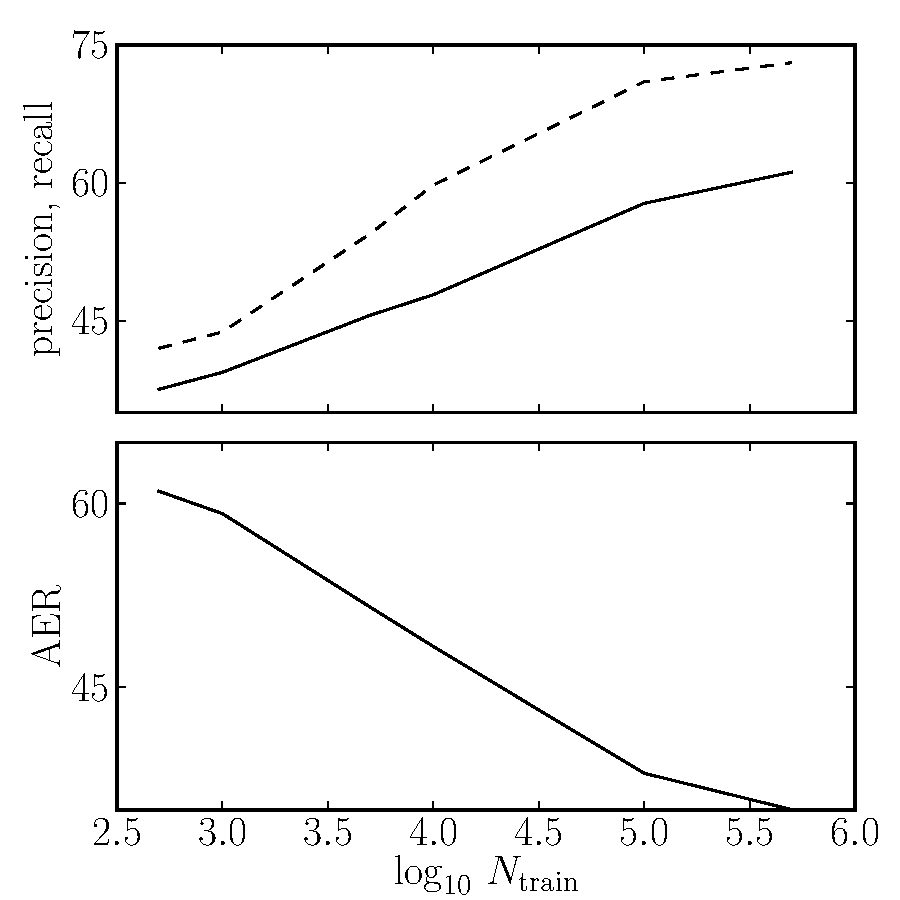
\includegraphics[width=0.5\textwidth]{heuristic.pdf}
\end{center}
\caption{%
The performance the heuristic word-alignment model on the validation dataset
as a function of the number $N_\mathrm{train}$ of training sentence pairs used.
The top panel shows the precision (solid line) and the recall (dashed line)
and the bottom panel shows the AER.
\figlabel{heuristic}}
\end{figure}

\section{IBM Model 1}

The next two models that I will consider are the first two models presented by
\citet{ibm}.
Both start from a particular factorization of \eq{prob}
\begin{eqnarray}
p(\bvec{f},\,\bvec{a}\,|\,\bvec{e}) &=&
    p(m\,|\,\bvec{e}) \, \prod_{i=0}^m p(a_i\,|\,m,\,l)\,p(f_i\,|\,e_{a_i})
    \quad.
\end{eqnarray}
Note that this equation is \emph{not} as general as \eq{prob}.
In particular, the main independence assumptions that go into this
factorization are that (a) the alignment probabilities are conditionally
independent given (only) the sentence lengths and (b) the translation
probabilities for each word pair are independent of the other words in the
sentence.
These are clearly brutal assumptions (especially given what we've learned
already in this course) but they do make the problem tractable.
We'll actually go one step further \citep[following][]{ibm} and assume the
prior probability on the French sentence length is a small (irrelevant)
constant $p(m\,|\,\bvec{e}) \equiv \epsilon$.
For \emph{Model 1}, we'll make the further assumption that the alignment
probabilities are uniform across the whole sentence
\begin{eqnarray}
p(a_i\,|\,m,\,l) &=& \frac{1}{1+l} \quad.
\end{eqnarray}
With these assumptions, the probabilistic model that we want to learn is
\begin{eqnarray}
p(\bvec{f},\,\bvec{a}\,|\,\bvec{e}) &=&
    \frac{\epsilon}{1+l}\,\prod_i p(f_i\,|\,e_{a_i}) \quad.
\end{eqnarray}
In practice, I included the \code{NULL} token in each English sentence and
special cased the alignment to that position to have a constant prior
probability $P_\mathrm{NULL}$ of alignment.
I chose to set this to $P_\mathrm{NULL}$ using a not particularly scientific
set of experiments but the results don't seem to be very sensitive to this
value.
Under this model, the parameters $p(f_i\,|\,e_j)$ and
$p(f_i\,|\,\mathrm{NULL})$ can be learned using expectation maximization.
The steps are roughly as follows:
\begin{enumerate}
\item{Initialize the distribution}
\end{enumerate}


\begin{table}[htbp]
\begin{center}
\begin{tabular}{c ccc}
\toprule
$N_\mathrm{train}$ & precision [\%] & recall [\%] & AER [\%] \\\midrule
500 & 35.098 & 35.799 & 64.665 \\
1000 & 38.427 & 41.420 & 60.573 \\
5000 & 52.000 & 55.030 & 46.964 \\
10000 & 55.522 & 58.876 & 43.343 \\
100000 & 60.602 & 63.314 & 38.485 \\
500000 & 64.363 & 67.160 & 34.681 \\
\bottomrule
\end{tabular}
\end{center}
\caption{%
The performance IBM Model 1 on the validation dataset
as a function of the number $N_\mathrm{train}$ of training sentence pairs used.
\label{tab:model1}}
\end{table}

\begin{figure}[htbp]
\begin{center}
    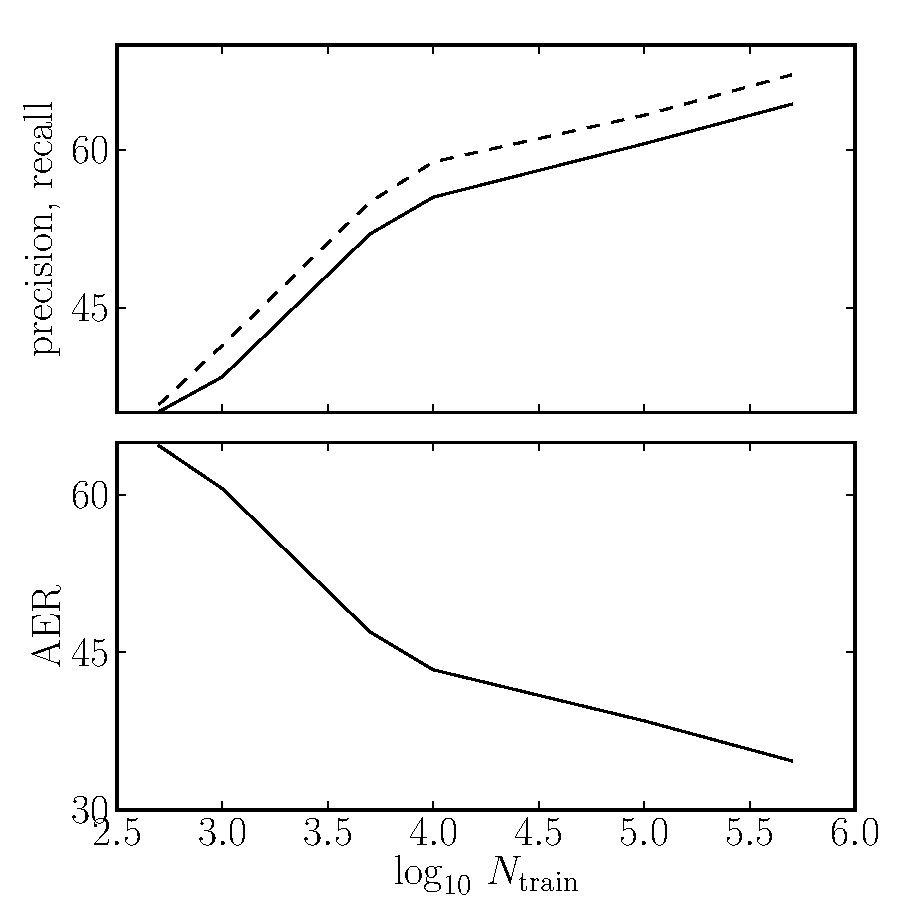
\includegraphics[width=0.5\textwidth]{model1.pdf}
\end{center}
\caption{%
\figlabel{model1}}
\end{figure}

\begin{figure}[htbp]
\begin{center}
    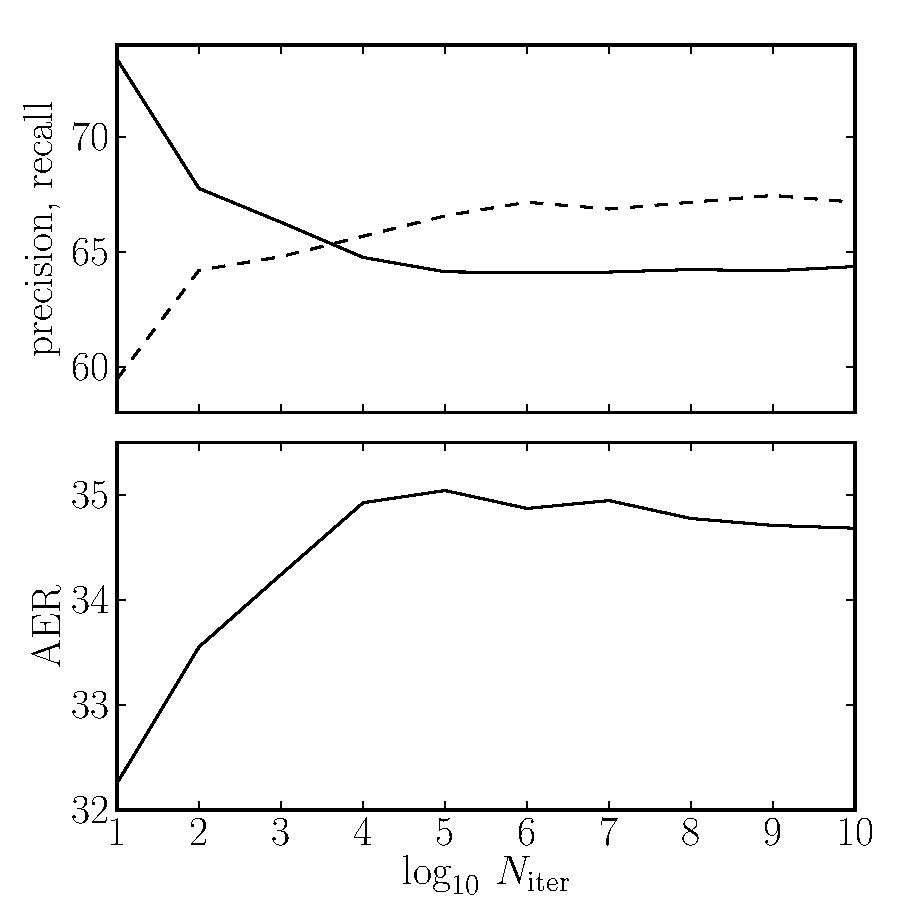
\includegraphics[width=0.5\textwidth]{model1_convergence.pdf}
\end{center}
\caption{%
\figlabel{model1-convergence}}
\end{figure}

\begin{table}[htbp]
\begin{center}
\begin{tabular}{c ccc}
\toprule
$N_\mathrm{train}$ & precision [\%] & recall [\%] & AER [\%] \\\midrule
500 & 48.451 & 56.805 & 48.855 \\
1000 & 55.603 & 65.385 & 41.199 \\
5000 & 63.329 & 76.923 & 32.283 \\
10000 & 65.678 & 78.698 & 30.115 \\
100000 & 69.448 & 81.953 & 26.507 \\
200000 & 71.469 & 84.024 & 24.474 \\
500000 & 73.371 & 84.320 & 23.084 \\
\bottomrule
\end{tabular}
\end{center}
\caption{%
The performance IBM Model 2 on the validation dataset
as a function of the number $N_\mathrm{train}$ of training sentence pairs used.
\label{tab:model2}}
\end{table}

\begin{figure}[htbp]
\begin{center}
    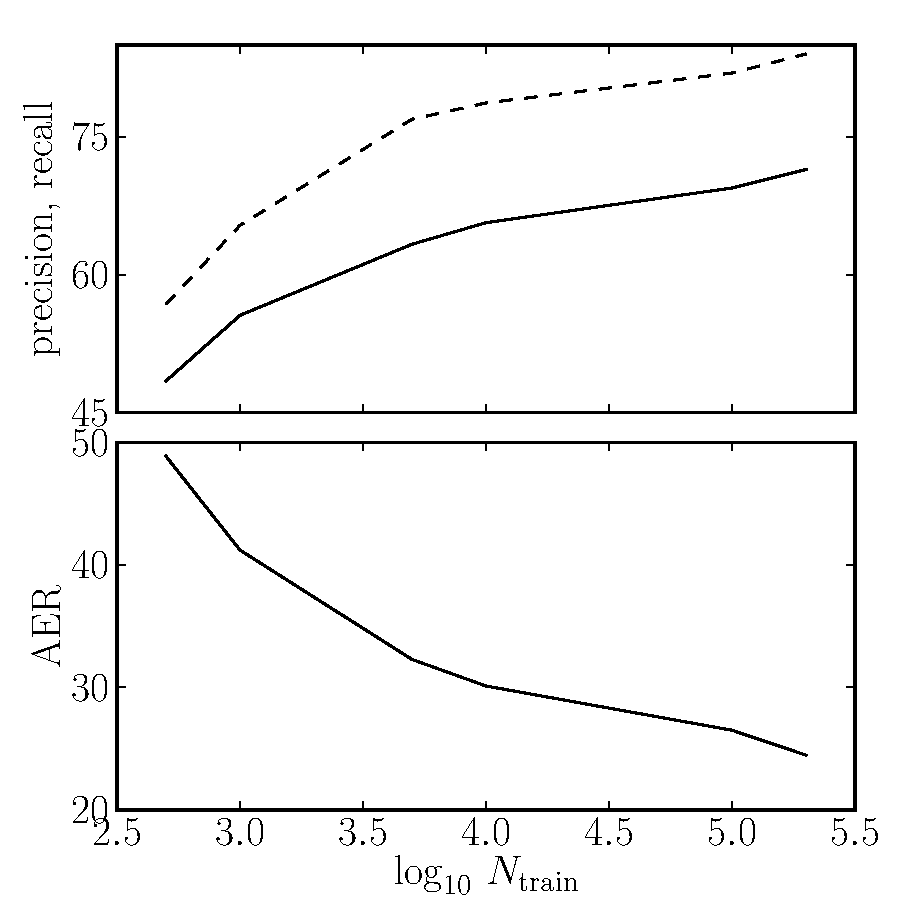
\includegraphics[width=0.5\textwidth]{model2.pdf}
\end{center}
\caption{%
\figlabel{model2}}
\end{figure}

\begin{figure}[htbp]
\begin{center}
    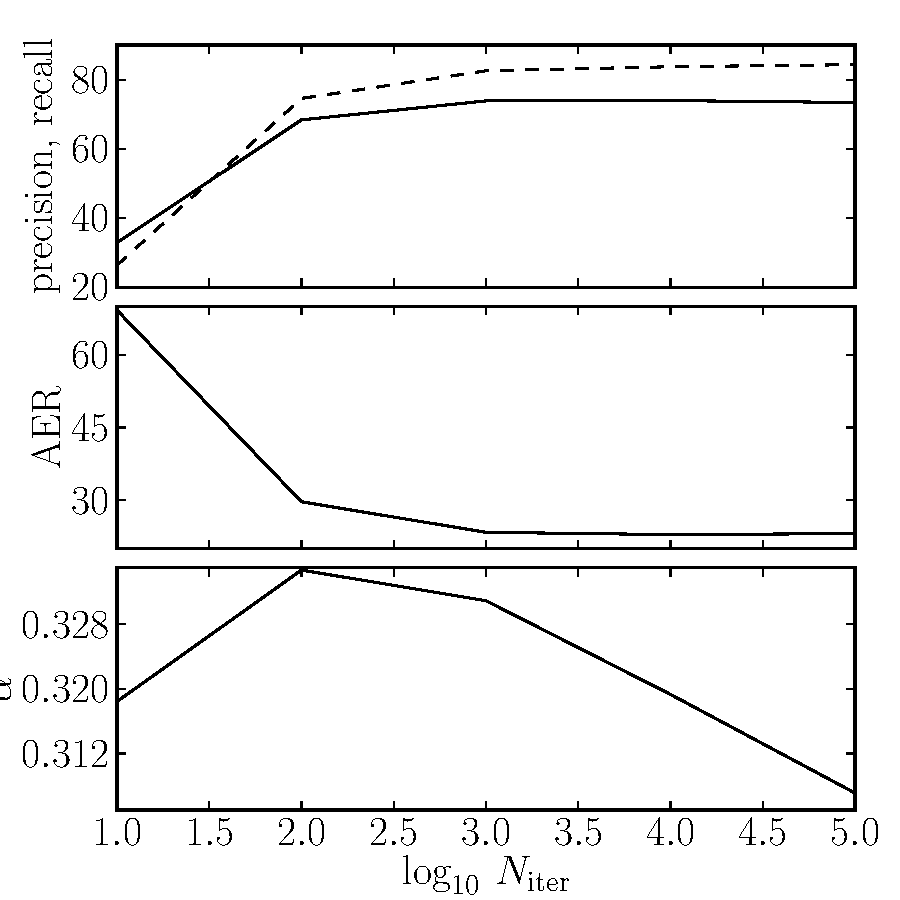
\includegraphics[width=0.5\textwidth]{model2_convergence.pdf}
\end{center}
\caption{%
\figlabel{model2-convergence}}
\end{figure}

\begin{thebibliography}{}\raggedright

\bibitem[Brown \etal(1993)]{ibm}
P.~F.~Brown, S.~A.~Della\ Pietra, V.~J.~Della\ Pietra, \& R.~L.~Mercer (1993)
\textbf{The Mathematics of Statistical Machine Translation: Parameter
        Estimation}, Computational Linguistics, 19, 2

\end{thebibliography}

\end{document}
